\chapter{Identifying Multiview Effects in Subsets of a Population}

\section{Introduction}

Most of the existing methods from multiview machine learning for combining different views of data assume that there is a latent structure common to the whole dataset for example the population lying on a normative spectrum of disease. However the truth may be more complex with some subjects having entirely different sources of variation and possibly even some anomalous subjects. In this chapter, we address the problem of finding multiple associations between views of data when each given sample may contain none, one, or any number of the associations (where we hypothesize that associations between the brain and clinical assessments are driven by or represent mental health variations). In order to tackle this problem, an algorithm must be able to identify both whether a sample contains a given association as well as the nature of the association (i.e. its associated weights). 

One way to formalise this problem is that we would like to build models which have sparsity over subjects or in other words some subjects contribute nothing to the objective in a similar way to how weights sparsity means that some features do not contribute to the objective. When there are two classes with different, but strong associations, classical methods will instead tend to combine the two associations into a shared, weaker association since subject sparsity is not built into the PCA, PLS, or CCA models. This is problematic both for interpreting the association and for separation of different conditions in a mental health context.

Progress on this work has so far been limited to understanding existing approaches to the problem and preliminary research on methods for addressing the problem. 

\section{Related Work}
\label{Related Work}

There have been a handful of approaches to the CCA problem that induce sparsity over samples. The sparse kernel CCA of \cite{chu2013sparse} finds sparse dual vectors in each view in order to improve robustness of the model by regularisation and to improve efficiency of inference at test time. \cite{fern2005correlation} developed a model with a similar philosophy to k-means clustering, with iterative reassignment between clusters and learning cluster parameters based on minimisation of some criterion. Like k-means clustering, this method requires an a priori assumption about the number of clusters and an assumption that there is a correlation between the views for all samples. 

\subsection{A metamorphosis of Canonical Correlation Analysis into Multivariate Maximum Margin Learning}

\cite{szedmak2007metamorphosis} developed a convex optimisation problem which is related to both the CCA problem and the one-class SVM. 

They start with the Rayleigh Quotient form for CCA:

\begin{align}
    & \bold{w_{opt}}=\underset{\bold{w}}{\mathrm{argmax}}\{\frac{ \bold{w_x^{\top}X^{\top}Yw_y } }{\|\bold{Xw_x}\|\|\bold{Yw_y}\|}\}\\
\end{align}

\begin{align}
    \bold{w_{opt}}=\underset{\bold{w}}{\mathrm{argmax}}\{\frac{\left\langle\mathbf{Y}, \mathbf{X} \mathbf{w}_{x} \mathbf{w}_{y}^{T}\right\rangle_{F}}{\|\mathbf{Y}\|_{F}\left\|\mathbf{X} \mathbf{w}_{x} \mathbf{w}_{y}^{T}\right\|_{F}}\}=\underset{\bold{w}}{\mathrm{argmin}}\{\frac{\|\mathbf{Y}\|_{F}\|\mathbf{X} \hat{\mathbf{W}}\|_{F}}{\langle\mathbf{Y}, \mathbf{X} \hat{\mathbf{W}}\rangle_{F}}\}\\
\end{align}

\begin{align}
    \bold{W_{opt}}=\underset{\bold{W}}{\mathrm{argmin}}\{ \|\mathbf{X}\mathbf{W}\|_{F}\} \\
    \text{subject to:} \notag\\ 
    \langle\mathbf{Y}, \mathbf{X} \mathbf{W}\rangle_{F} \geq 1
\end{align}


Before finally proposing a solution with a soft margin. In the case that the data dependence in $\|X_2W\|_F$ is ignored in place of $\|W\|_F$ (an assumption similar to the regularisation effect of PLS with respect to CCA):

\begin{align}
    & \bold{W_{opt}}=\underset{\bold{W}}{\mathrm{argmin}}\{\|\bold{W}\|^2_F + C\bold{1}^{\top}\xi\}\\
    & \text{subject to:} \notag\\
    & \bold{x^{(i)}_2 W x^{(i)}_1}  >=1-\xi_i \notag\\
\end{align}

By considering the slack variables $\xi_i$ as indicators of samples lacking the underlying correlation, this method can be used to select samples which do not share the correlation by considering those with $\xi_i > 0$ as negative samples.

\subsection{Sample Weighted PLS}\label{Sample Weighted PLS}
\cite{wenwen2018sparse} develop what they call a weighted sparse CCA method which learns a sparse sample weight vector as well as the weight vectors for each view which allows them to learn a model of a signal which exists in some samples but not others. This is described by the optimisation problem:

\begin{align}
    & \bold{w_{opt}}=\underset{w}{\mathrm{argmax}}\{ \bold{w_1^{\top}X_1^{\top}\text{diag}(d)X_2w_2  }\}\\
    & \text{subject to:} \notag\\
    & \bold{w_1^{\top}w_1}=1 \notag\\
    & \bold{w_2^{\top}w_2}=1 \notag\\
    & \bold{d^{\top}d}=1 \notag
\end{align}

Which they suggest to solve by alternating optimisation over $\bold{w_1}$ and $\bold{w_2}$. Their algorithm is performant on certain types of data but has a tendency to have large weights (the elements of $\bold{d}$) on a small subset of the samples rather than selecting all of the correlated samples more uniformly. In addition the constraints on $\bold{w_i}$ are PLS constraints rather than CCA constraints implying an assumption of diagonal covariance. For this reason in comparison we will refer to this algorithm as Sparse Weighted PLS. Finally, they show that in principle we can further regularise the weights since it only changes the subproblems in the alternating minimisation.


\subsection{Correlation Clustering}\label{sec:corrclus}

The final algorithm we review here is the correlation clustering algorithm from \cite{fern2005correlation}. The basic steps of the algorithm are somewhat like the expectation maximisation algorithm for k-means clustering. The algorithm alternates between a model fitting step in which $k$ CCA models are fit 

\vspace{\baselineskip}
\begin{algorithm}
\begin{algorithmic}[1]
\STATE {Finds regression model parameters which best fit the data}
\STATE {$k=$ maximum iterations}
\STATE {$n=$ minimum number of samples in each fit, typically the minimum number required by the model e.g. the number of parameters for regression}
\STATE {$t=$ threshold for point to be considered well fit}
\WHILE {iterations $< k$}
    \STATE Randomly assign instances to the $k$ clusters.
    \STATE For $i=1 \cdots k$, apply CCA to cluster $i$ to build $M^{i}=\left\{\left(u_{j}, v_{j}\right), r_{j},\left(a_{j}, b_{j}\right): j=1 \cdots d\right\}$, i.e., the top $d$ pairs of canonical variates, the correlation $r$ between each pair, and the corresponding $d$ pairs of projection vectors.
    \STATE Reassign each instance to a cluster based on its $\vec{x}$ and $\vec{y}$ features and the $k$ CCA models.
    \STATE If no assignment has changed from previous iteration, return the current clusters and CCA models. Otherwise, go to step 2 .
\ENDWHILE
\caption[Correlation Clustering]{Correlation Clustering}
\label{alg:Correlation Clustering}
\end{algorithmic}
\end{algorithm}

\section{Contributions}

\begin{itemize}
    \item \textbf{Contribution 1:} Formulating PCA, PLS and CCA as Maximum Margin Robot formulations and considering how they can be used to select population subsets containing the relevant signal
    \item \textbf{Contribution 2:} An adjusted form of the Weighted PLS from section \ref{Sample Weighted PLS} based on alternating optimisation with better convergence properties
\end{itemize}

\section{\textbf{Contribution 1:} Maximum Margin Robots for Dimensionality Reduction in the Presence of Outliers}

\subsection{Maximum Margin PCA}

Since our interest in the maximum margin formulation of CCA to identify which samples contain the signal of interest, it is interesting to first study the (arguably) simpler problem of PCA to better understand the properties of the Maximum Margin Robot and the types of scenarios where it is most effective. We can write a PCA 

\begin{align}
    & \bold{W_{opt}}=\underset{W}{\mathrm{argmin}}\{\|\bold{W}\|^2_F + C\bold{1}^{\top}\xi\}\\
    & \text{subject to:} \notag\\
    & \bold{x^{(i)} W x^{(i)}}  >=1-\xi_i \notag\\
\end{align}

\subsection{Maximum Margin CCA}

Similarly, we can add back in the data dependence to the Maximum Margin Robot for PLS to give a CCA-like problem.

\begin{align}
    & \bold{W_{opt}}=\underset{W}{\mathrm{argmin}}\{\|\bold{X_1WX_2^{\top}}\|^2_F + C\bold{1}^{\top}\xi\}\\
    & \text{subject to:} \notag\\
    & \bold{x^{(i)}_1 W x^{(i)}_2}  >=1-\xi_i \notag\\
\end{align}

\section{\textbf{Contribution 2:} An Improved Sparse Weighted CCA}

The constraints defined by \cite{wenwen2018sparse} assume the same approximation as the Penalized Matrix Decomposition described earlier. For this reason, their method is better understood as a form of Sparse Weighted PLS. If we substitute these constraints for the true CCA constraints, the problem can still be solved to a local optimum by alternating optimisation:

\begin{align}
    & \bold{w_{opt}}=\underset{\bold{w}}{\mathrm{argmax}}\{ \bold{w_1^{\top}X_1^{\top}\text{diag}(d)X_2w_2}  \}\\
    & \text{subject to:} \notag\\
    & \bold{w_1^{\top}X_1^{\top}X_1w_1}=1 \notag\\
    & \bold{w_2^{\top}X_2^{\top}X_2w_2}=1 \notag\\
    & \bold{d^{\top}d}=1 \notag
\end{align}

However this method inherits the weaknesses of the Sparse Weighted PLS with respect to the vector $\bold{d}$, namely that this constraint has a tendency toward a peaky distribution with a very large weight on a small number of samples. For this reason, we consider the following change to the constraint:

\begin{align}
    & \bold{w_{opt}}=\underset{\bold{w}}{\mathrm{argmax}}\{ \bold{w_1^{\top}X_1^{\top}\text{diag}(d)X_2w_2}  \}\\
    & \text{subject to:} \notag\\
    & \bold{w_1^{\top}X_1^{\top}X_1w_1}=1 \notag\\
    & \bold{w_2^{\top}X_2^{\top}X_2w_2}=1 \notag\\
    & 0\leq d_i \leq 1 \notag
\end{align}

Once again this problem can be solved by alternating optimisation of $w_1$, $w_2$, and $d$. In this case, the elements of $d$ will be either 0 or 1 depending if the projections for a given sample have a positive product or a negative product.

\section{Experimental Results}

Work so far has been an iterative process of understanding the existing methods as well as investigating their performance in different kinds of simulated data.

In all of the experiments we generate a strong `signal of interest' for a population and add a noisy population without an interesting signal. The goal in our constructions is to successfully recover the correct subspace of the interesting population, ideally by simultaneously classifying subjects as interesting or non-interesting. 

Hyperparameters are approximately tuned to the correct region (e.g. ensuring that not all of the slack variables are zero or all slack variables are active) but not optimized. This is because firstly it is not clear what a good optimization criteria would be and secondly it allows us to explore the properties of the algorithms while avoiding cherry picking.

\subsection{PCA}

\subsubsection{Experiment Design}

In the PCA experiments, we generate data by combining two datasets with the same total variance (sum of eigenvalues). The first, interesting, dataset has a much larger first eigenvalue while the second uninteresting dataset has equal eigenvalues. PCA will naturally tend to combine the largest signals in both datasets. We generate 100 interesting samples and 50 uninteresting samples with 10 features.

We show plots of the the data projected onto the first two `principal components' identified by each model in order to demonstrate how well they capture the true subspace. We provide a ground truth by running PCA on only the interesting samples. We show projections for both the training data as well as held out test data.

In addition we show plots of the effective sample weights for each model. Since each model formulates the problem in a slightly different way we highlight that this means:

\begin{itemize}
    \item PCA: the absolute value of the score of each sample or the rows of $Xw$ where $w$ are the weights that form the first principal component. This is motivated by the fact that samples which are projected to near zero contribute very little to the PCA objective.
    \item MMR: Since the model uses slack variables to allow for low variance samples, we obtain `sample weights' by subtracting these slack variables from 1. This means a sample with a zero slack variable has sample weight equal to one. A sample with a maximal slack variable equal to one would have a sample weight of zero.
\end{itemize}

\subsubsection{Results}

The results in figures \ref{fig:pcalatent} and \ref{fig:pcaweights} show that classical PCA is highly effective at suppressing the low variance data, with the uninteresting 'random' samples all clustered around the centre of the PCA subspace while the interesting 'signal' samples form much of the variance. Nonetheless, an interesting property of MMR is that it fairly cleanly assigns 0 slack variables to the vast majority of the interesting samples giving a clean classification. 

\begin{figure}[H] 
    \centering
    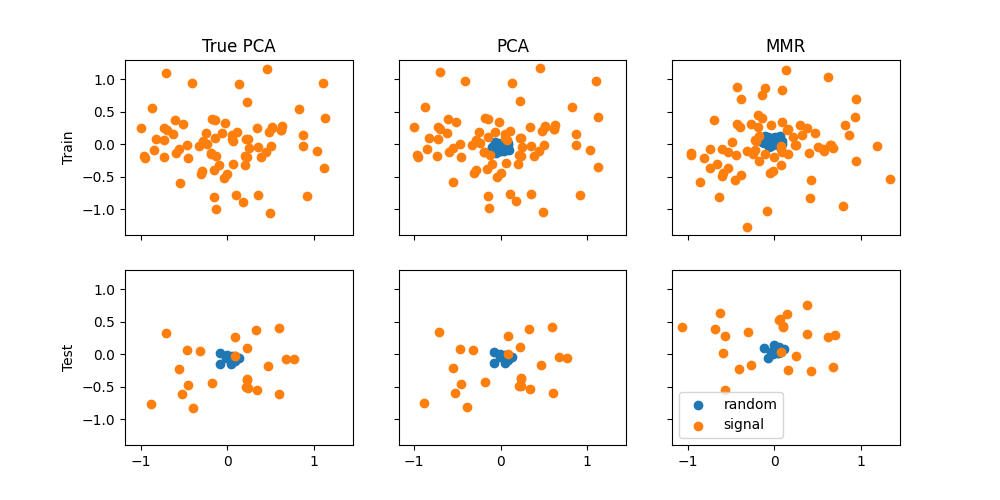
\includegraphics[width=0.9\textwidth]{chapters/sampleselection/pca/models.png}
    \caption{Plots of the first two `principal components' estimated by each model on the x and y axis. The leftmost model is trained using only the interesting data and therefore presents a ground truth}
    \label{fig:pcalatent}
\end{figure}

\begin{figure}[H] 
    \centering
    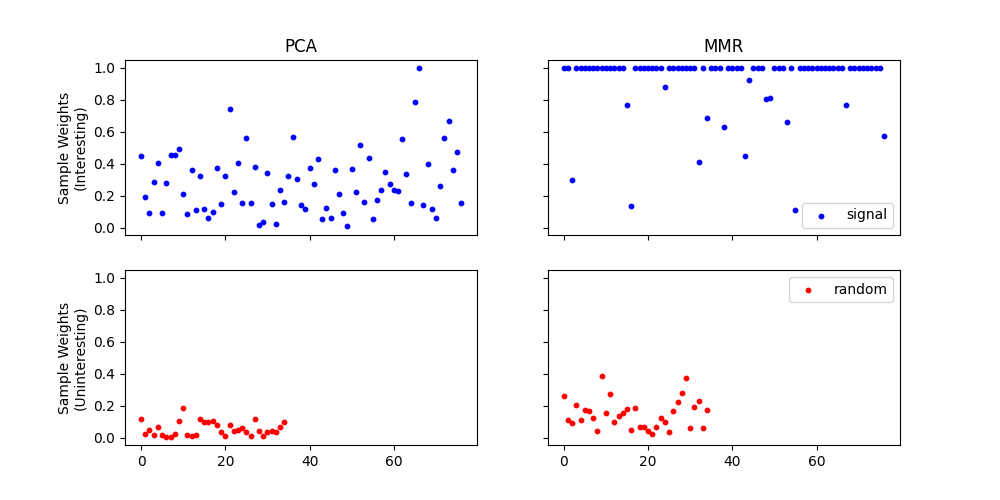
\includegraphics[width=0.9\textwidth]{chapters/sampleselection/pca/weights.png}
    \caption{Plots showing the implied sample weights by both models with the rows separating the interesting samples (top) from the uninteresting samples (bottom). An ideal model would have all samples=1 in the top row and all samples=0 in the bottom.}
    \label{fig:pcaweights}
\end{figure}

\subsection{PLS}

\subsubsection{Experiment Design}

In the PLS experiments, we generate data by combining two multiview datasets. The first is generated using Witten's method described in chapter \ref{chap:framework} while the latter is random noise with the same columnwise variance as the first dataset. We generate 100 interesting samples and 50 uninteresting samples with 10 features in two different views.

One major weakness of using Witten's latent variable model to generate the data with a signal is that the samples associated with the smallest values in the latent variable vector will have lower variance in the data and it is clearly impossible to distinguish between arbitrarily small latent variables and data generated without the latent variables.

We show plots of two views projected onto their first highly covarying latent dimension. We provide a ground truth by running PLS on only the interesting samples. We show projections for both the training data as well as held out test data. The goal for any model is to maximise the covariance of the projections of the `interesting' data.

In addition we show plots of the effective sample weights for each model. Since each model formulates the problem in a slightly different way we highlight that this means:

\begin{itemize}
    \item PLS: The sample wise product of the projections of each view $X_1w_1$ and $X_2w_2$. This is motivated by the fact that samples which drive the covariance objective are those where the projections have the same sign and a large magnitude.
    \item MMR: Since the model uses slack variables to allow for low variance samples, we obtain `sample weights' by subtracting these slack variables from 1. This means a sample with a zero slack variable has sample weight equal to one. A sample with a maximal slack variable equal to one would have a sample weight of zero.
    \item WPLS: The elements of the vector $\bold{d}$ provide a natural sample weighting in their formulation
    
\end{itemize}

\subsubsection{Results}

The results shown in figures \ref{fig:plslatent} and \ref{fig:plsweights} show a degree of promise for using methods which induce sparsity over samples in the PLS context. MMR in particular appears to better suppress the random data when compared to PLS in the latent plots. Interestingly, this is less clear from the sample weighting plots. Our variant of WPLS does not appear to perform well in this context in the sense of successfully recovering the sample weights.

\begin{figure}[H] 
    \centering
    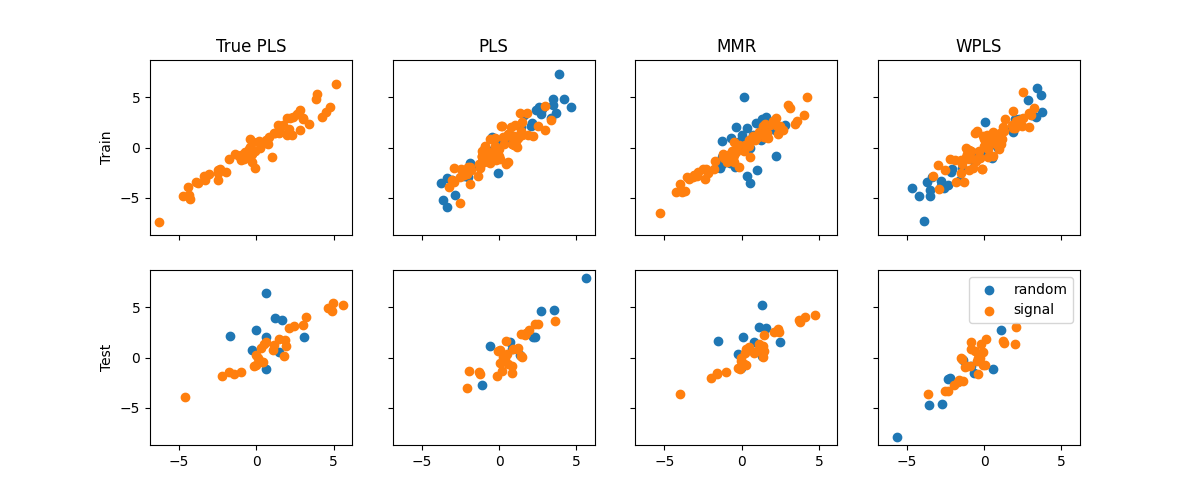
\includegraphics[width=0.9\textwidth]{chapters/sampleselection/pls/models.png}
    \caption{Plots of the first latent score for each view plotted against each other as a scatter plot. The leftmost model is trained using only the interesting data and therefore presents a ground truth}
    \label{fig:plslatent}
\end{figure}

\begin{figure}[H] 
    \centering
    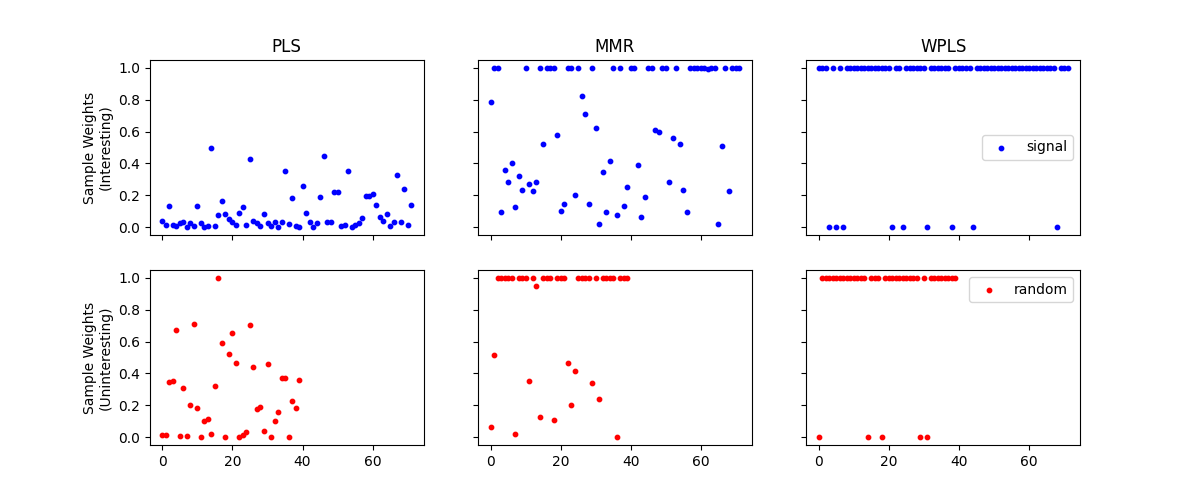
\includegraphics[width=0.9\textwidth]{chapters/sampleselection/pls/weights.png}
    \caption{Plots showing the implied sample weights by both models with the rows separating the interesting samples (top) from the uninteresting samples (bottom). An ideal model would have all samples=1 in the top row and all samples=0 in the bottom.}
    \label{fig:plsweights}
\end{figure}

\subsection{CCA}

\subsubsection{Experiment Design}

In the CCA experiments, data generation follows the same scheme described for the PLS experiments.

We show plots of two views projected onto their first highly correlated latent dimension. We provide a ground truth by running CCA on only the interesting samples. We show projections for both the training data as well as held out test data. The goal for any model is to maximise the correlation of the `interesting data'.

In addition we show plots of the effective sample weights for each model. Since each model formulates the problem in a slightly different way we highlight that this means:

\begin{itemize}
    \item PLS: The sample wise product of the projections of each view $X_1w_1$ and $X_2w_2$. This is motivated by the fact that samples which drive the covariance objective are those where the projections have the same sign and a large magnitude.
    \item MMR: Since the model uses slack variables to allow for low variance samples, we obtain `sample weights' by subtracting these slack variables from 1. This means a sample with a zero slack variable has sample weight equal to one. A sample with a maximal slack variable equal to one would have a sample weight of zero.
    \item WCCA: The elements of the vector $\bold{d}$ provide a natural sample weighting in their formulation
    \item Cluster Correlation: In a binary problem with two groups, we can use the binary classification as a sample weight for visualisation purposes.
\end{itemize}

\subsubsection{Results}

The results shown in figures \ref{fig:ccalatent} and \ref{fig:ccaweights} once again imply some promise for sample selection algorithms. In particular, classical CCA appears to have been driven somewhat by the random data while WCCA and ClusterCorrelation appear to project the interesting samples to a more correlated latent space. The poor performance of MMR suggests a problem with our implementation or construction but is presented for completeness.

\begin{figure}[H] 
    \centering
    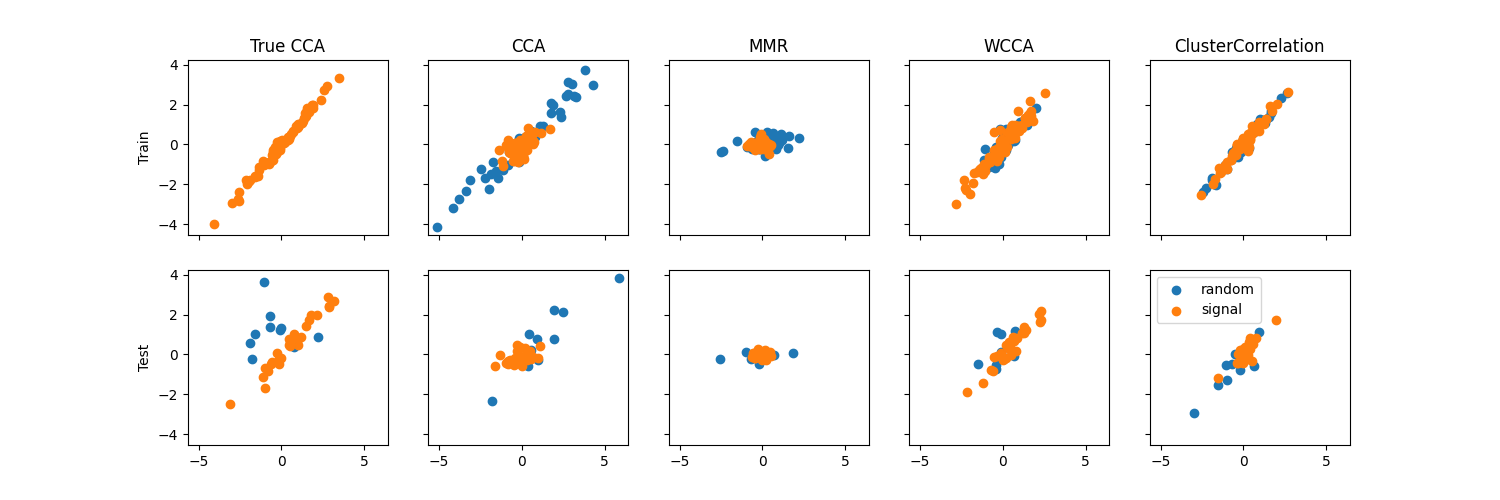
\includegraphics[width=0.9\textwidth]{chapters/sampleselection/cca/models.png}
    \caption{Plots of the first latent score for each view plotted against each other as a scatter plot. The leftmost model is trained using only the interesting data and therefore presents a ground truth}
    \label{fig:ccalatent}
\end{figure}

\begin{figure}[H] 
    \centering
    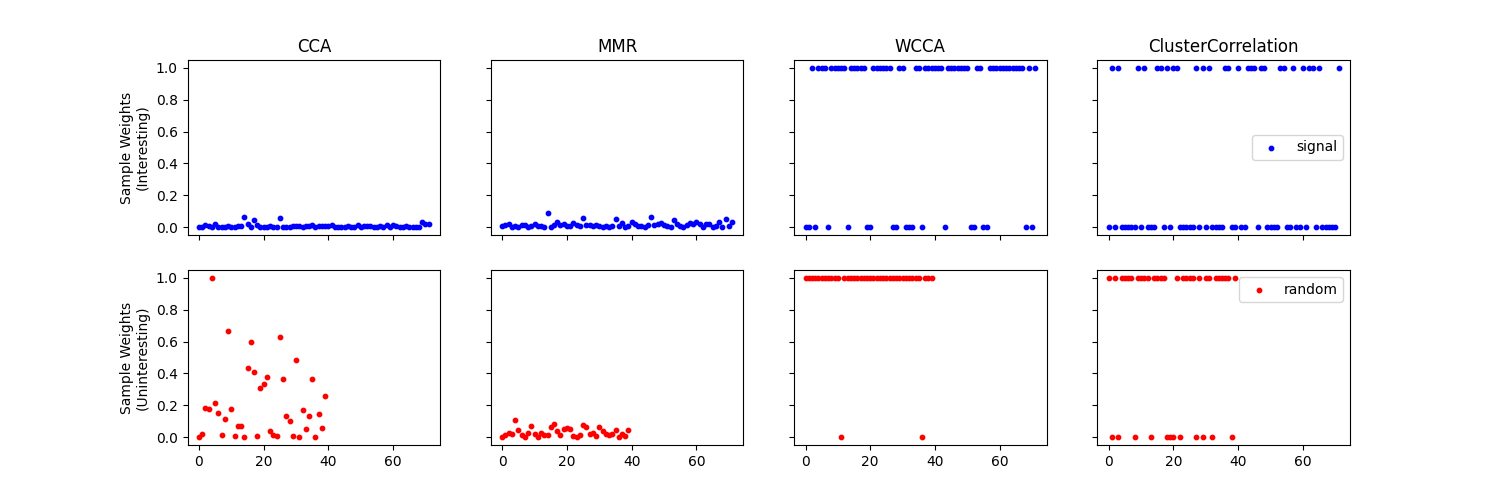
\includegraphics[width=0.9\textwidth]{chapters/sampleselection/cca/weights.png}
    \caption{Plots showing the implied sample weights by both models with the rows separating the interesting samples (top) from the uninteresting samples (bottom). An ideal model would have all samples=1 in the top row and all samples=0 in the bottom.}
    \label{fig:ccaweights}
\end{figure}

\section{Future Work}

This project remains at a somewhat exploratory stage so much of the future work will need to identify situations where these methods could be valuable.

\subsection{Application to GENFI Dataset}

This dataset has the interesting property of containing ground truth subtypes which could be used to validate any promising models. Recent work using Group Factor Analysis \cite{Ferreira2021} has shown promise extracting meaningful brain-behaviour associations using a probabilistic model and upcoming work by the same authors uses probabilistic model with sparsity over subjects. This provides a useful benchmark for our work.

